\chapter{Results and discussions} \label{chapter5}

The following subsections shall discuss in detail, a variety of important comparisons which affect the project work, a brief overview of the methodologies learned, deviations from the ideal case (if any) and a creator’s road map for implementation of a similar project and other moderate and small details. It also has a section for the work which is being currently done at SEBI to improve the existing system. The initial two sections deal with metrics of accuracy and execution time across two different bases for comparison while the section that follows discusses why the metrics are chosen and defined as they are. \par

\section{Comparison between OCR models} \label{comp_ocr}

Both Tesseract and EasyOCR are sophisticated OCR engines and are available as open-source in their default versions. However, there exists an outsized number of differences in how they have been developed. While Tesseract \cite{Google2015} happens to be a quite superior alternative right from the beginning which can use even PDF files as input apart from the standard images, it turns out that there doesn’t exist any suitable interface with common programming languages (such as Python) which leads to a lot of problems. The first and foremost problem is that Tesseract needs to be set up in a way similar to how a particular program is set up on a remote server i.e. the \textit{only link} between a program using Tesseract and the actual engine is the file path. Customisations can be done nonetheless, but are difficult to implement due to the lack of a high-level interface. This leads directly to another issue: the Ezmeral MLOPs platform is set up on a legacy Centos 7.5 virtual machine cluster and won’t allow arbitrary software to be installed in it due to the presence of an enterprise-grade security architecture.  So it may be the better OCR engine in general, however, this use case is unsuitable for it.\par

EasyOCR offers as many capabilities \cite{Jaided2020} as Tesseract (\textit{sans} the direct processing of PDF files) and has a \textbf{high-level} library directly available for use in Python. This means that no preliminary server like set-up needs to be done to access the OCR engine, rather everything is on board once the program and all its imported modules are loaded onto memory. Hence, EasyOCR was chosen as the OCR for this project. \par

It should be noted that EasyOCR is a ready-to-use OCR that is invariant to colour images while the Tesseract documentation does say things about providing a greyscale image as input. This feature alone avoided a lot of extra image processing operations within the codebase. After using EasyOCR, the following changes took place:

\begin{itemize}
 \item The size of the codebase was greatly reduced (from $1400$ lines to less than $1000$ lines).
 \item The execution time dropped significantly (from $73$ to $14$ minutes: a reduction of $\approx 80\%$ on similar environments).
 \item Major improvements were not visible in accuracy although EasyOCR still managed to perform better ($A_{e} = 0.94375$ and $A_{e} = 0.95$ respectively).
\end{itemize}

Amongst all decoded values at the end of a particular run, the following results were obtained and are summarised below.

\begin{figure}[h]
  \centering
  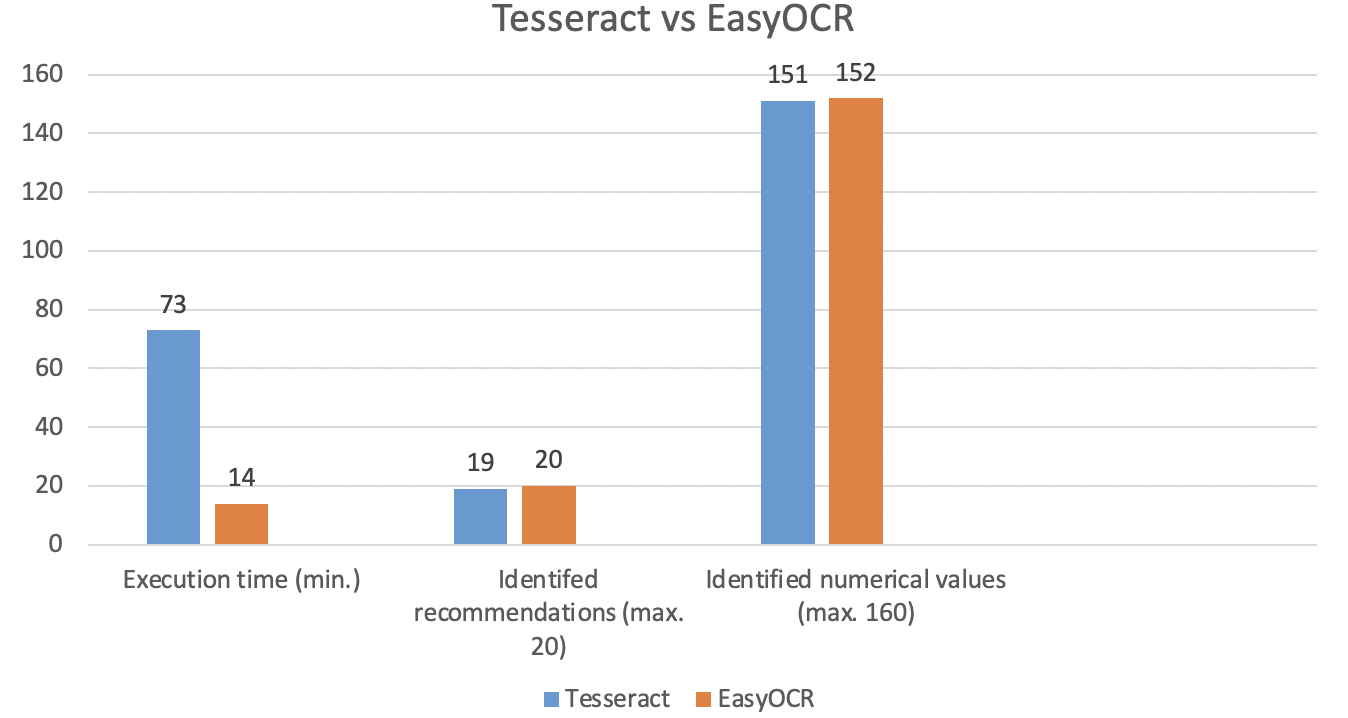
\includegraphics[scale=0.7]{chapter5/barchart.png}
  \caption{Comparison of Tesseract and EasyOCR for a sample $30$ minutes telecast}
  \label{fig:easy_vs_tess}
\end{figure}

Still, EasyOCR (and the project) benefits even further from a possible change in hardware configuration which is detailed in the following section.


\section{Comparison between hardware architectures}

It is a known fact that almost all deep learning systems (inclusive of computer vision models) benefit greatly from the presence of GPUs in the development environment. Although as of now the Ezmeral cluster doesn’t have GPU access, testing was still performed on a local workstation with an \href{ https://www.nvidia.com/en-in/geforce/20-series/}{RTX 2060} graphics card with the equivalent Nvidia \href{https://developer.nvidia.com/cuda-toolkit}{CUDA toolkit} installed. \par

It should be noted that \textbf{no execution environment} discussed earlier in chapter \ref{chapter4} had any mention of GPUs so there was a decrease in execution time by a large margin for the same test video. The decrease of roughly by a factor of $4.5$ w.r.t. to the closest competitor i.e. for execution recorded on a standalone VM. The reason for this was obvious: the documentation of EasyOCR mentions that their pipeline is more performant in the presence of a GPU \cite{Jaided}. The results are summarised in the form of a bar chart below.

\begin{figure}[h]
  \centering
  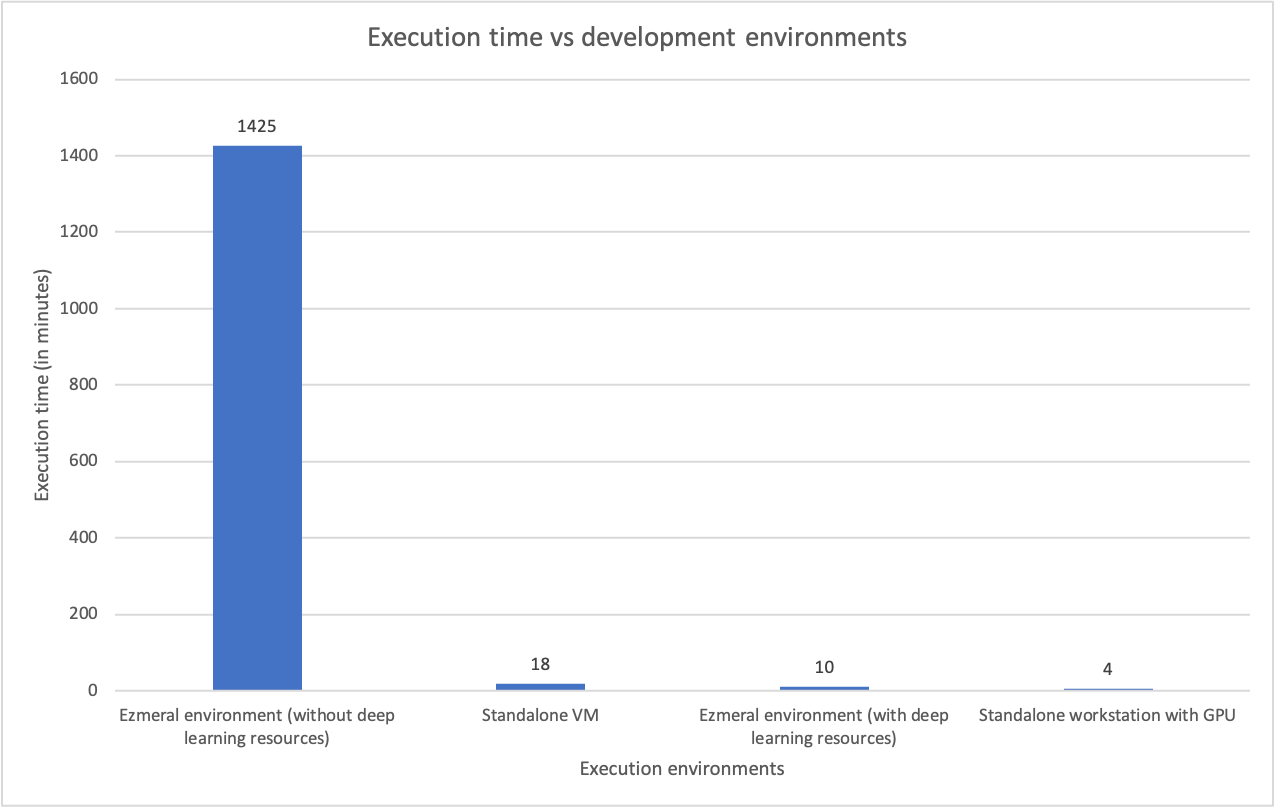
\includegraphics[scale=0.7]{chapter5/barchart2.png}
  \caption{A comparison of execution times across a variety of development environments with a variety of hardware configurations}
  \label{fig:hardware}
\end{figure}

\section{Current workflow progress and testing procedures}

\subsection{Workflow progress}

As stated in earlier chapters, the work at hand is to process a total of $7$ NEWS shows in their entirety (excluding only one for the lack of recommendations in it) to summarise all the recommendations being provided in them. This shall ensure that when more sophisticated anomaly detection models are run on them, the input (produced as an output from my project) is sufficient for them to run properly. Additionally, it should also be noted that the systems succeeding the ones used in this project also use several data cleaning procedures before arriving at a final output so a \textit{picture-perfect output is not necessary although desirable}. \par

The following table lists the shows on one side and the percentage of total videos of each show that has been processed.

\begin{table}[h]
 \def\arraystretch{1.5}
 \centering
 \caption{Batch workflow progress}
 \begin{tabular}{|c|c|}
  \hline
  NEWS show & Progress (in \%)\\
  \hline
  Buy Now Sell Now & $10$                   \\
  \hline
  Pehla Sauda & $25$                   \\
  \hline
  NSE Closing Bell & $10$                   \\
  \hline
  Bazaar Morning Call & $10$                   \\
  \hline
  Midcap Bazaar & $35$                 \\
  \hline
  Stock 20-20 & $100$                \\
  \hline
  Weekly Roundup & \textbf{Omitted}               \\
  \hline
 \end{tabular}
 \label{tab:news_prog}
\end{table}


\subsection{Testing procedures}

Usually, there are no clearly defined testing procedures for such custom projects in deep learning and computer vision. A typical testing procedure that was used to verify the authenticity and the accuracy of the output is that after filtering out frames at the FPS rate, the recommendations being made in a \textit{handful} of videos were noted down manually. This was then compared to the output obtained from the program. If there is a perfect match (which was mostly the case), then the output is deemed to be suitable otherwise \textbf{no separate improvements} are made midway in a batch processing workflow. The reason for this is two-fold:

\begin{enumerate}

 \item Batch processing workflows involve a very large number of videos at once, stopping them in between drastically decreases the efficiency of such workflows and the more important reason being

 \item Anomaly detection systems or models which follow this project already employ sufficient data cleaning procedures to obtain a reliable and usable output within tolerable error limits.

\end{enumerate}

\section{Accuracy}


\section{Inferences and learnings}

\subsection{Possible usage of only an OCR engine}

It would be worthwhile to reason why an OCR engine is not directly used on the extracted frames since it would detect the required text followed by which the programmer is supposed to consolidate it to a usable form. \par

The reason lies in the abilities of EasyOCR as an OCR engine which is both an advantage as well as a disadvantage. It should be known that, unlike Tesseract which uses page segmentation modes \cite{Rosebroc2021} to detect text in an image structurally arranged in specific configurations, EasyOCR doesn’t have any such facility. It directly returns a list of bounding box coordinates, the text detected along with a confidence score across the entire image \cite{Jaided}. The above is an illustration of what might happen if numerous texts were provided to EasyOCR on a signboard.

\begin{figure}[h]
  \centering
  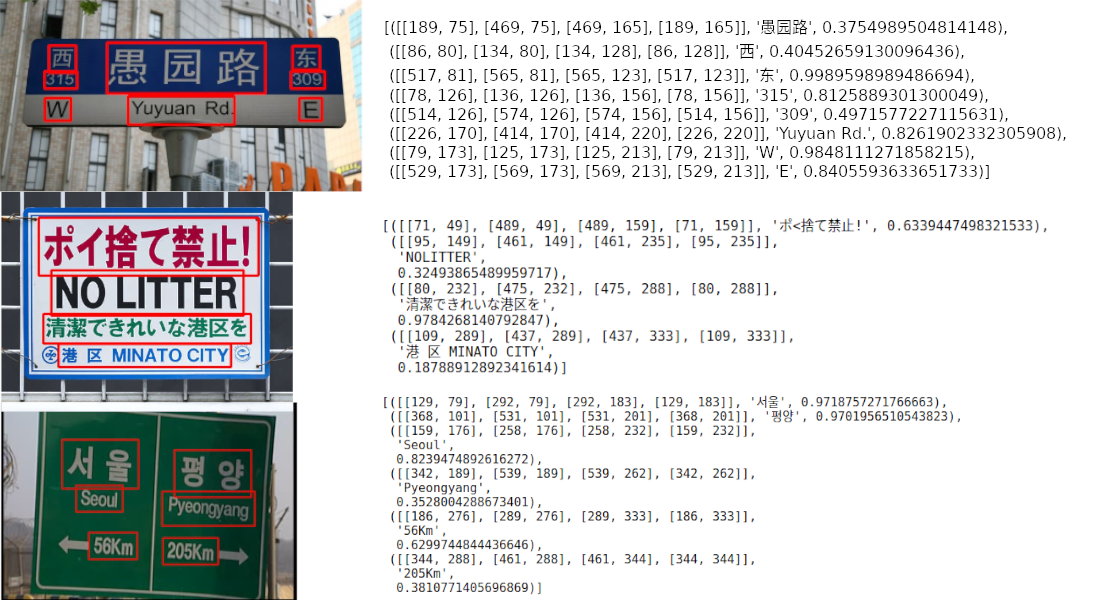
\includegraphics[scale=0.45]{chapter5/example2.png}
  \caption{Execution of EasyOCR on three signboards}
  \label{fig:easy_signboard}
\end{figure}

We would realise that all texts scattered throughout the image are returned, however, we are unable to draw any correlation between them at first look. This could prove to be a major challenge in this project wherein multiple related numerical and alphanumeric values are placed close to each other. In an extreme case where multiple recommendations are detected in the same frame, it would be very difficult to detect the mapping of the numerical values (such as stop-loss or target price) and the listing symbol of a company share. Hence, the choice of using an object detection model followed by an OCR engine.

\subsection{Procurement of data from a contractor}

It has been clearly stated in section \ref{vid_data} that the entirety of the video data was obtained from \href{clipbyte.com}{Clipbyte}. It would be worthwhile to argue that all videos could be directly downloaded from a platform like \href{youtube.com}{YouTube}. However, there are two major reasons for not doing so:
\begin{enumerate}
 \item All broadcasts of the concerned NEWS shows are not available on such video platforms and nor do the respective channels upload videos in a timed and orderly manner.

 \item There is no official way to download videos from such a platform so availing videos from such a platform by a Government regulatory body would imply improper means of accessing publicly available information in the situation wherein the InVestigations Department (IVD) of SEBI has to file a case against a suspected entity. The data source needs to be mentioned in the case file and hence a separate contractor has been tended for this job.

\end{enumerate}



\section{Accuracy, empirical accuracy and execution time}

A lot has been discussed about the various performance metrics used to evaluate object detection models in section \ref{metrics}, however, we still stick to the concept of simple empirical accuracy in the above two sections. The reason for the same is that there are multiple ML/DL models which are involved in this project. Each model has been designed (or is being used) to complete only a specific task amongst a large number of tasks that are to be executed sequentially. Each task involves different kinds of data and hence produces different kinds of output. \par

A simple e.g. being that the YoLo models discussed throughout the report output a set of mixed values as given in section \ref{brief_discuss} after taking in an image as an input. However, the OCR models that follow require an image as an input, but produce a textual output (i.e. of string datatype). These models within them have two deep learning models i.e. a \textit{text detection} and a \textit{language} model in a cascaded fashion out of which only the former receives an input in the form of an image while the second model deals with textual input and output. \par

Each of these models named above has its own set of accuracy metrics which may be discussed however, they would be irrelevant to the final output of the project. Hence, we have stuck to the concept of simple empirical accuracy which is defined by the set of values obtained at the end from the OCR and summarised in the CSV file and is defined as follows

\begin{equation}
\centering
A_{e} = 1 - \frac{No. \ of  \ NA \ values \ in \ the \ CSV}{Total \ no. \ of \ values \ in \ the \ CSV }
\end{equation}

\textit{Measuring execution time remains the same i.e. in seconds although at a couple of places wherein the execution time is large, seconds have been replaced by larger units of time}. \newpage

\section{Sample outputs}

This section has a couple of outputs for multiple NEWS shows for the sake of reference to the reader.

\begin{figure}[h]
  \centering
  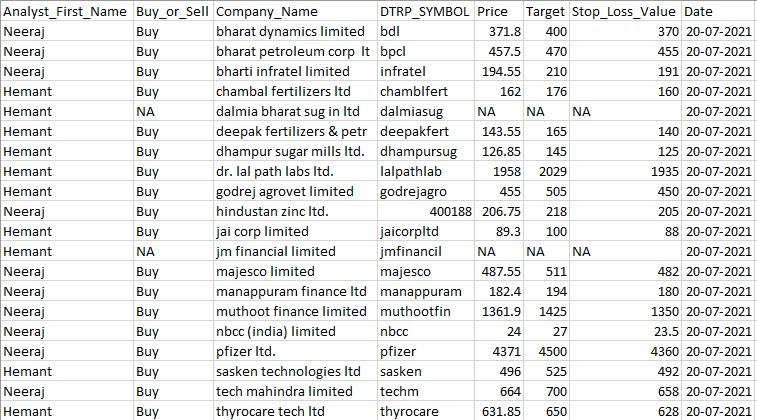
\includegraphics[scale=0.7]{chapter5/output csv.jpeg}
  \caption{The output file obtained for the broadcast of the NEWS show Stock 20-20 on 20/07/2021}
  \label{fig:out1}
\end{figure}

\begin{figure}[h]
  \centering
  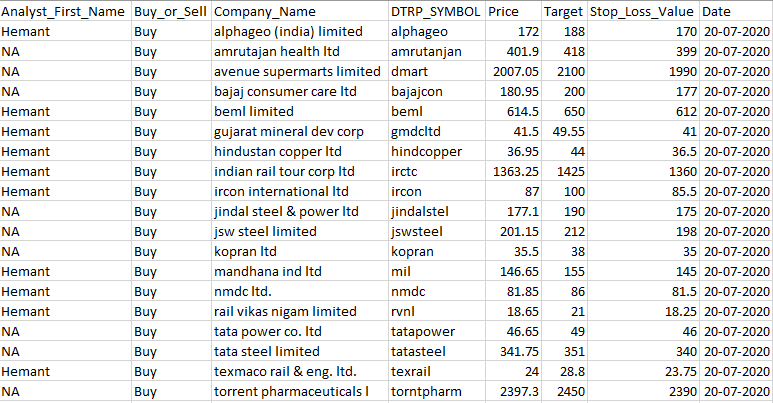
\includegraphics[scale=0.7]{chapter5/output2 csv.png}
  \caption{The output file obtained for the broadcast of the NEWS show Stock 20-20 on 20/07/2020}
  \label{fig:out2}
\end{figure} \newpage

\begin{figure}[h]
  \centering
  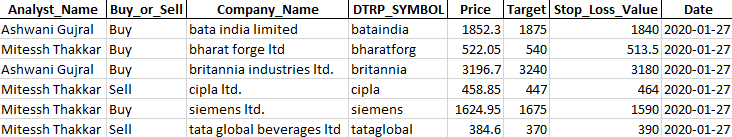
\includegraphics[scale=0.7]{chapter5/output3 csv.png}
  \caption{The output file obtained for the broadcast of the NEWS show CNBC TV18 on 27/01/2020}
  \label{fig:out3}
\end{figure}


\section{Future work}

The current system can be improvised in two different areas as given below. A workflow improvement can also be made.

\subsection{Accuracy and efficiency}

The current system does filtering at only the FPS rate which manages to reduce the number of frames under consideration to a much smaller value (a $25$\textsuperscript{th} of it to be precise). However, as we have seen in chapter \ref{chapter3}, the frame selection is still not inherently intelligent and still leads to the production of  $ \approx 1400$ frames on an average, amongst which frames would be manually selected for annotation. \par

Theoretically, we can say that for the problem statement at hand; there exists a program $P$ that extracts and processes exactly $N$ frames such that the total no. of recommendations being made, $R$ is contained in exactly $N$ keyframes. \par

To do so we can use an adaptive frame extraction algorithm \cite{adapt} which shall extract only the frames which are important to us. This method is based on matching histograms of successive frames, a correlation that exists amongst their colour channels, etc. This shall greatly reduce the number of frames to be processed at a time (apart from the already existing FPS rate filtering). This method, however, could be tending to fail because similar-looking frames \textit{need not be redundant} to us just because they appear close to each other in the actual video. In that case, we can go for an alternative approach wherein the frame numbers are output according to a simple implementation of any multi-output regressor \cite{Brownlee2020}. Since there could be inherent inaccuracies in the training of the same, we can use a spreading factor $\Delta$ which shall extract keyframes starting from ${f}_{k} - \Delta$ to ${f}_{k} + \Delta$ instead of just the frame $f_k$.

\subsection{Usability}

Currently, a two-part deployment and its necessity are deemed to be confusing to many SEBI officers who work in the surveillance department and don’t have any prior programming knowledge. Both these deployments could be integrated into a single native cross-platform desktop app developed either using \href{https://riverbankcomputing.com/software/pyqt/intro}{PyQt} or \href{electronjs.org}{Electron} which shall have an intuitive front end design and the same set of calling scripts as its backend. This shall help concerned officers keep track of ongoing workflows as well as use them when required without interfering with ongoing batch workflows and being aware of the complexity of the ML/DL code behind it.

\subsection{VM workflow} \label{future}

The landing server of SEBI Datalake would soon be modified in a way that it will subscribe to an MRSS feed on the Clipbyte platform wherein any new video once pushed shall automatically trigger a workflow. The VM workflow would be modified accordingly so that it either runs as a \href{https://en.wikipedia.org/wiki/Cron}{\textbf{cron}} job at scheduled intervals or it executes only when a new video is available for processing.
